%-*- coding: utf-8 -*-
\subsection{MenuGen}
\begin{figure}
  \centering
      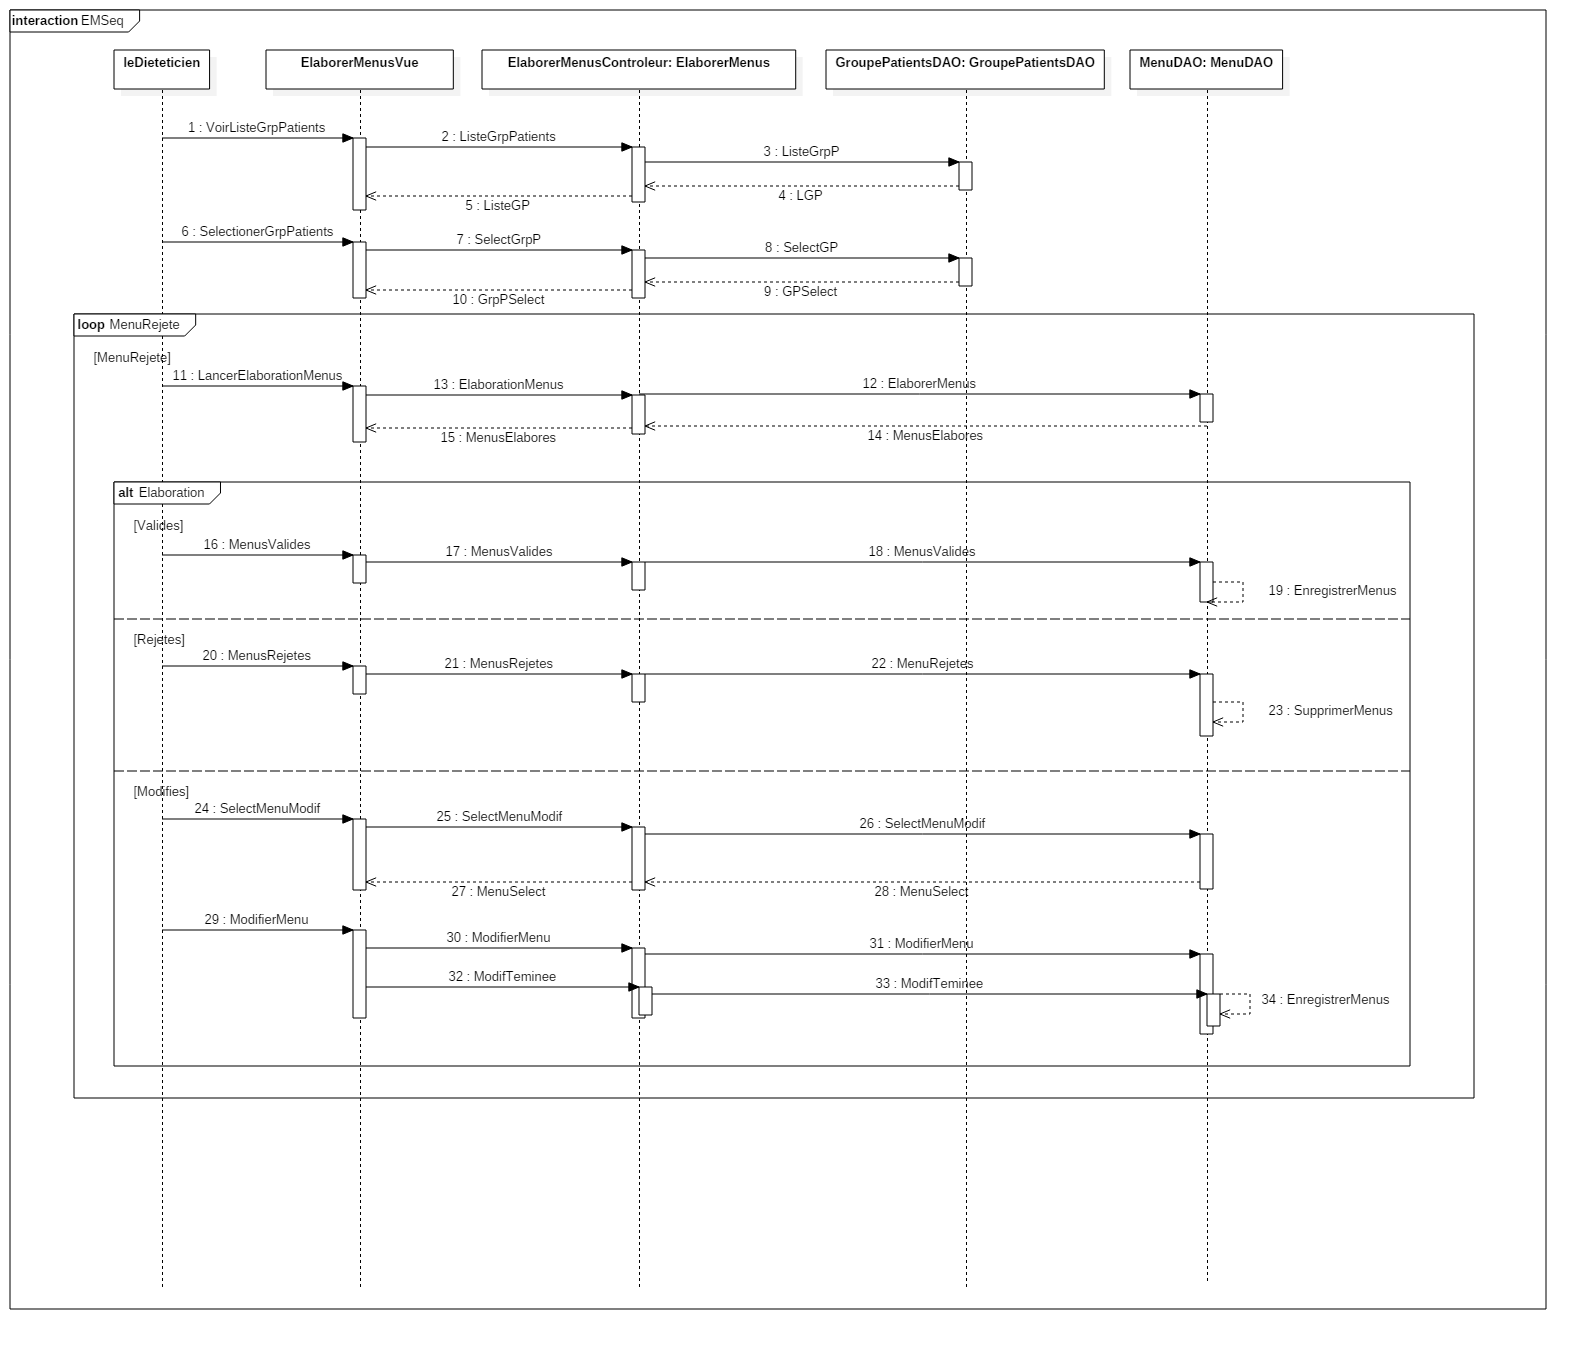
\includegraphics[width=1.00\textwidth]{../../CasDUtilisations/MenuGen/Sequence/EMSeq.png} %
\caption{Séquence détaillée d'élaboration des menus}
\label{MenuGenSeqDetail}
\end{figure}

\textbf{Algorithme (voir \autoref{ClassesMenuGen}):}
\begin{enumerate}
\item Sélectionner le groupe de patient dont il faut élaborer les menus
\item Extraire de ce groupe de patients les contraintes sous forme d'une table d'\emph{AttributAliment} (voir \autoref{ModeleDuDomaine}).
\item Générer une table contenant en plus des identifiants de plats la liste de leurs ingrédients, sous forme d'\emph{AttributAliment}.
\item Retirer de cette table, les plats incompatibles avec les contraintes listées dans la première table.
\item En comparant la table de plats résultante avec les menus déjà pris, extraire de la liste des plats (première table) les plats compatibles avec les fréquences de services.
\item élaborer les menus à partir de la liste des plats restants.
\end{enumerate}

\begin{figure}
  \centering
      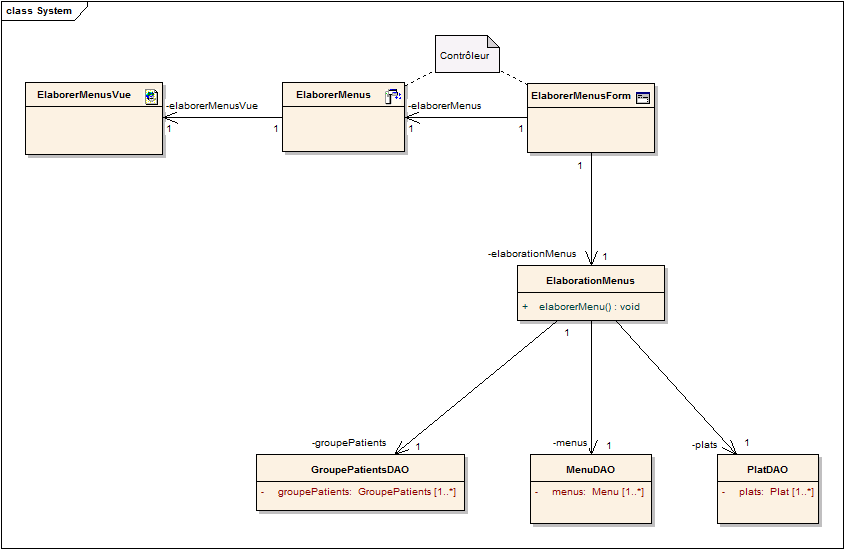
\includegraphics[width=1.00\textwidth]{../../CasDUtilisations/MenuGen/Classes/EMC.png} %
\caption{classes d'élaboration des menus}
\label{ClassesMenuGen}
\end{figure}
